\section{Advantages, Limitations, and hybrid algorithms}
\label{sec:comparison}

As should be evident from the preceding sections, each technique has its own strengths and weaknesses: e.g., the simplicity in the formulation of counterdiabatic driving comes at the price of the often highly complex control terms it necessitates, optimal quantum control produces high-fidelity protocols so long as it does not get stuck in local minima, whereas the ability of RL agents to generalize typically requires large amounts of data. In Table~\ref{table:comparisons} we provide our opinion on some of the key advantages and limitations for each of the approaches discussed in Secs.~\ref{sec:STA}-\ref{sec:RL_theory}.

\begin{table}[h!]
\centering
\begin{tabular}{|p{2.5cm}|p{5.5cm}|p{5.5cm}|p{1.5cm}|}
\hline
Techniques & Advantages \& focus & Limitations \& Scope of applicability & References \\
\hline
\hline
\multicolumn{4}{|c|}{\textbf{Shortcuts-to-adiabaticity} -- Sec.~\ref{sec:STA}} \\
\hline
\hline
Counterdiabatic driving & Analytically derived which guarantees effectiveness and also allows \steve{us} to provide physical insight into fundamental controllability of the system & Only strictly applicable to exactly solvable models and often results in highly nonlocal control terms limiting direct experimental implementability & Refs.~\cite{STAreview,Berry2009} \\
\hline
Variational counterdiabatic driving & Can be approached semi-analytically or fully numerically and lends itself to a hybrid approach combined with quantum optimal control. Allows \steve{us} insight into the adiabatic gauge potential in regimes where its exact calculation is difficult. & The local approximation of counterdiabatic terms tends to be poor when approaching critical and/or transition points in the spectrum, i.e., where energy gaps close. & Ref.~\cite{sels2017minimizing,kolodrubetz2017geometry} \\
\hline
\hline
\multicolumn{4}{|c|}{\textbf{Quantum optimal control} -- Sec.~\ref{sec:QOC}} \\
\hline
\hline
Open-loop optimal control & Systematic approach that can be applied to any setting and allows \steve{us} to impose physically motivated constraints, e.g. allowable operations, time scale etc. Benign landscape structure gives certain guarantees to find good, if not necessarily the absolutely optimal, solution & Does not generalize as system parameters change - each configuration requires solving a new optimization problem. Numerically obtained control solutions are hard to interpret physically. & Refs.~\cite{Glaser2015} \\
% \hline
% Closed-loop (feedback) control & Can or should we say something here? & and here? & Refs \\
\hline
\hline
\multicolumn{4}{|c|}{\textbf{Machine Learning based quantum control} -- Sec.~\ref{sec:RL_theory}} \\
\hline
\hline
Reinforcement Learning & Versatile in scope of application and like OC can accommodate any constraints from the outset. Can generalize to unseen setups (e.g., starting from different initial states). (Typically) does not require gradients of the function to be optimized. Does not require information about the controlled quantum system. & May require a lot of training data. (Typically) does not come with formal convergence guarantees. May get stuck in a suboptimal local minimum. Does not require information about the controlled quantum system. & Refs~\cite{GiannelliPLA} \\
\hline
Other ML~approaches & Train once, apply in diverse setups. Whenever optimization is time-consuming, learn the correct optimized output to avoid running it every time. & Generalization (i.e., extrapolation and interpolation) has limits and depends on the data used in training. Requires static training data distribution (i.e., characteristic system parameters should not change over time). & Refs.~\cite{mehta2019high,carleo2019machine} \\
\hline
\end{tabular}
\caption{Comparative table highlighting some key advantages and limitations of the various control techniques presented throughout the tutorial and other closely related approaches.}
\label{table:comparisons}
\end{table}

While we have presented and discussed each control technique in isolation, with an aim to provide a clear pedagogical introduction to the basic mathematical formulation of quantum control protocols, it is worth highlighting that significant benefits can be achieved by {\it combining} these techniques together. The effectiveness of such an approach can already be seen in fairly rudimentary settings e.g. Sec.~\ref{ex:LMGmodel} where counterdiabatic driving informed the choice of operators to employ for the control, leaving the pulse shape to be optimised. More sophisticated approaches, although similar in spirit, have been used to control many-body systems by combining shortcuts-to-adiabaticity with optimal control to design more experimentally favourable control protocols. The most intuitive approach starts by constraining the available set of controllable operators. By optimising the operators' time dependence, this technique can allow for remarkably good performance when traversing a critical point~\cite{Saberi2014, CampbellPRL} so long as we stay away from the thermodynamic limit when the spectral gap closes and the norm of the AGP diverges. As we will discuss more below, variational counterdiabatic driving allows \steve{us} to formalise and significantly expand this approach as shown in Ref.~\cite{COLD_PRXQ}. Beyond the clear practical advantage that hybrid approaches can provide vis-\'a-vis designing easier to implement control protocols, it can also allow to explore the fundamental limits of controllability. Hybrid control approaches allow to determine the true minimal control time under a given set of constraints and, therefore, explore the attainability of fundamental bounds such as the quantum speed limit and Lieb-Robinson bounds~\cite{Kiely2021NJP, Kiely2022PRR}. Significant efficiencies in the optimisation procedure itself are also attainable by combining gradient-free with gradient-based optimisation procedures~\cite{KochEPJQT2015}, the crucial insight here being that once the need for numerical optimisation enters the problem, it can be highly advantageous to ensure that a `good' initial seed is employed. This becomes particularly relevant when exploring rugged control landscapes~\cite{Chakrabarti2007, Beato2024a, Beato2024b, Fentaw2025}.

For the other considered control techniques, as we have seen, both optimal control and reinforcement learning offer numerical tools to devise quantum control protocols, and a natural question arises as to when one gains an edge over the other. A major difference between RL and optimal control is that optimal control focuses on the optimal solution and any acquired information about the physical system used during optimization is lost. RL, on the other hand, extracts essential information for maximizing the reward, and stores it in the policy -- a left-over product. Reinforcement learning algorithms are capable of re-using this information at a later stage, e.g.~starting from a different initial state, self-correcting for exploration mistakes made during training or caused by noise/uncertainty, or even trying to control a related but different system. However, this comes at a cost: RL is not computationally as efficient as optimal control and takes more iterations to find an optimal solution, especially if it starts without prior knowledge of the controlled system (cf.~model-free vs.~model-based RL~\cite{sutton_barto_rl}). Another advantage of RL over established quantum control methods, which rely on built-in optimization algorithms, is the balance between exploitation of already obtained knowledge, and exploration in uncharted parts of the control landscape (a.k.a.~the Exploration-Exploitation dilemma~\cite{sutton_barto_rl}, which was mentioned also in Sec. \ref{subsec:QOC_intro}). Below the quantum speed limit, decision-based exploration offers an alternative to multi-starting local gradient optimizers. Unlike such methods, the RL agent progressively becomes familiar with the control landscape, and finds protocols robust to sampling noise. Due to exploration noise, RL is not suitable for finding global minima of the cost function; in return, the minima it finds are more stable/robust to changes in the protocol. In difficult optimization problems, however, optimal control is never guaranteed to find the globally optimal protocol either, and we usually have no way of verifying if it did. Anticipating possible future applications of RL in physics, we note that RL brings in three key ideas:
(i) \emph{model-free} RL requires no pre-knowledge of the controlled physical system;
(ii) \emph{adaptive} RL transfers acquired knowledge to new setups and can point to hidden relations between nonequilibrium phenomena;
(iii) \emph{autonomous} RL provides novel insights into automating complex manipulation protocols. \\

Hybridized procedures allow to circumvent pitfalls associated with a particular approach, ultimately pushing the limits of controllability. As previously mentioned, a drawback of counterdiabatic driving (and associated analytical techniques) is the requirement to exactly solve the model, thus significantly limiting its range of applicability. However, it is evident that many physically relevant settings can be approximated by models with known analytical solutions. From the above examples and discussion, it follows that using the information accessible by determining the control protocol for the analytically tractable approximation, can serve as a highly insightful seed which can then be optimised using, e.g. optimal control theory and/or machine learning. Such an approach has already been demonstrated to be highly effective in a diverse range of settings, we refer the reader to Refs.~\cite{Hegade2022portfolio,Chandarana2023digitized,wurtz2022counterdiabaticity,yao2021reinforcement, Ref1}, for some further examples. 
%There has also been some success in improving approximations to counterdiabatic terms through the addition of control fields to enable the best path to be chosen from a family of dynamical Hamiltonians \cite{COLD_PRXQ,morawetz2024efficient}.
To highlight the benefit that hybridized control strategies offer we mention three recent approaches that are showing particular promise: 
\begin{itemize}
\item {\it Enhanced shortcuts-to-adiabaticity (eSTA)}. The analytical nature of STA methods means that they have typically been applied to low-dimensional, idealised models. Thus, while the models serve as approximations to real physical systems, it is evident that directly applying the corresponding control terms to the actual system would, necessarily, not achieve perfect finite-time adiabatic dynamics. However, given that the formulation of STA methods guarantees that a counterdiabatic control term exists, it follows that if the Hamiltonian description of the real physical system can be considered a perturbation away from the idealised model, the correct control term is also likely to be closely related to the one derived for the idealised model. This insight served as the starting motivation for eSTA techniques~\cite{eSTA1, eSTA2}, which combines the knowledge learned from the STA methods together with gradient based optimisation to achieve high fidelity control in several physically relevant settings, in particular transport~\cite{eSTA1, eSTA2, eSTA6} and expansion~\cite{eSTA3} in anharmonic trapping potentials, manipulation and transport in double well~\cite{eSTA7}, driven qubits beyond the rotating wave approximation~\cite{eSTA1}, and bosonic Josephson junctions~\cite{eSTA5}. The computed control terms have also been shown to be robust to systematic errors and noise sources~\cite{eSTA2, eSTA5}. 

\item {\it Counterdiabatic local optimised driving}. The approach of variational counterdiabatic driving introduced in Sec.~\ref{subsec:varl_AGP} enabled the construction of approximate CD terms through minimisation without the need to diagonalise the Hamiltonian \cite{sels2017minimizing,kolodrubetz2017geometry}. This minimisation procedure can be tackled analytically for a limited set of scenarios, including the Ising model discussed in Sec.~\ref{subsec:varl_AGP}, but often requires numerical minimisation protocols to obtain the coefficients of the approximate CD for a particular protocol, akin to those discussed in the context of quantum optimal control in Sec.~\ref{sec:QOC}. The most natural way to enhance the performance of variational CD protocols is to introduce higher-order CD terms with operators that involve more bodies, i.e., by adding up to $N$-body interactions, but these are inherently nonlocal and often difficult to engineer in experiments or on quantum hardware. Note, these nonlocal and many-body terms are also what we are precisely wanting to avoid calculating when motivating the introduction of variational counterdiabatic driving. Counterdiabatic local optimised driving~\cite{COLD_PRXQ} takes a different approach by fixing the variational CD at low, local, orders of approximation while adding control fields that extend the family of dynamical Hamiltonians that can be explored. This allows \steve{us to use} counterdiabatic optimised local driving to find the optimal dynamical path for the local approximated CD. Recent work has extended this to determine the additional control fields and associated optimal set of operators necessary for a given problem~\cite{morawetz2024efficient}. Furthermore, this approach allows one to optimise the dynamical protocol without direct simulation, by calculating the ignored nonlocal CD terms and minimising their contribution, and this method could be further enhanced by combining it with the numerical approaches that have since been developed to calculate the CD terms, which we will discuss in Sec.~\ref{subsec:numagp}.

\item As a framework providing optimization algorithms capable of learning, RL presents an ideal playground for developing concepts for hybrid quantum control. Whereas RL does not magically produce high-fidelity protocols, this can be greatly facilitated by combining it with various STA methods, including CD driving, explored in Refs.~\cite{yao2021reinforcement,XiChenRL1}. The key idea to apply RL to real-world NISQ devices is to exploit the Quantum Approximate Optimization Algorithm (QAOA) which defines a variational quantum circuit with unknown parameters. The RL agent has to learn either the gate angles (continuous) or the circuit architecture (discrete) and, ideally, both. Since solving both the continuous and discrete optimization involves mixed continuous-discrete action spaces which can be challenging to deal with, often one resorts to RL for one of these two problems, leaving the other to optimal control methods (Sec.~\ref{sec:QOC}), such as gradient descent, or tree searches~\cite{yao2022monte}. To design the circuit architecture ansatz, one can use the terms appearing in the nested commutator ansatz~\cite{Claeys2019Floquet} for the variational AGP, see Sec.~\ref{subsec:varl_AGP}. While this does not implement CD driving itself, these terms generate unitary dynamics that unlocks shortcuts in the Hilbert space, leading to efficient state preparation away from the adiabatic regime. 
Using this approach Ref.~\cite{yao2021reinforcement} developed RL agents to prepare ground states of many-body spin chains on NISQ devices, while the RL agent of Ref.~\cite{XiChenRL1} is trained to design optimal pulses for single-qubit gates applicable, e.g., on a superconducting qubit device. 
We have explored in detail such hybrid CD-RL control shortly, see Sec.~\ref{sec:RL_2q}.
We mention in passing that, besides CD driving, RL can be combined in a hybrid approach to optimize dynamical invariants -- a different STA technique~\cite{XiChenRL3}.
\end{itemize}

\clearpage

\section{Future challenges and prospects for quantum control}
\label{sec:Outlook}

The ubiquity of control means that the techniques and tools presented above can find fertile application in a wide variety of places. In this section, we conclude this tutorial by briefly touching on several areas where quantum control is prevalent and where there are potentially significant benefits to be gained from the continued development of more advanced techniques for coherent control of complex quantum systems, see Fig.~\ref{fig:outlook}.\\

\begin{figure}[h]
%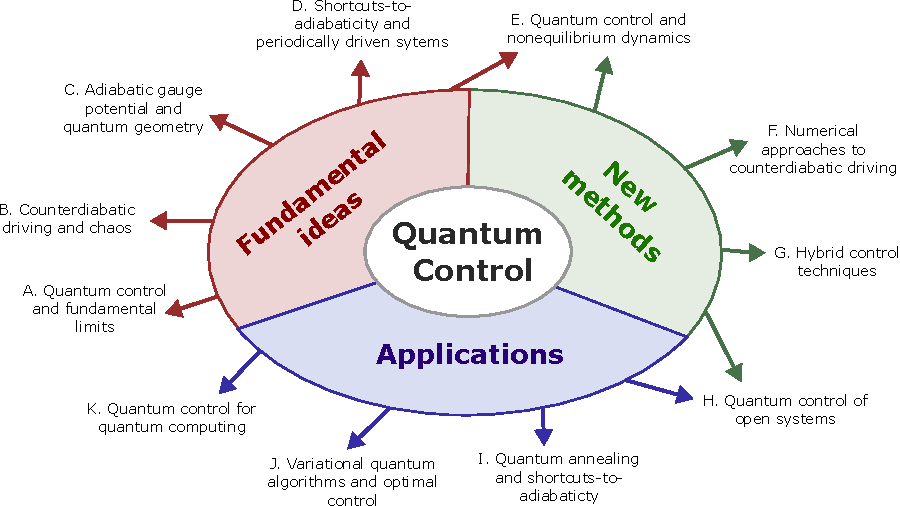
\includegraphics[width=0.8\columnwidth]{Fig_outlook.pdf}
%\vskip 1cm
\label{fig:outlook}
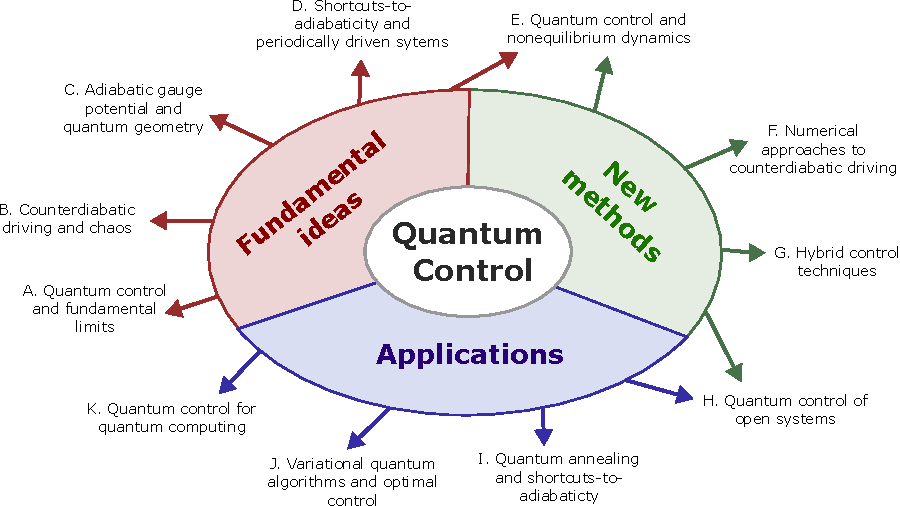
\includegraphics[width=0.85\columnwidth]{Fig_outlook.pdf}
\caption{Overview of the topics discussed in Sec.~\ref{sec:Outlook} and their relation to fundamental ideas, new methods, and applications of quantum control tools.}
\end{figure}

\subsection{Quantum control to push fundamental limits in quantum dynamics}
Given a model for a quantum-dynamical system and a target state or unitary transformation, the tools of optimal control allow us to search for a protocol that achieves such a process. If the optimization systematically fails to find a solution, this could indicate that the process was not achievable, with the resources available, in the first place, thus revealing a fundamental limitation of the dynamics. In the examples of Sec. \ref{sec:QOC}, this was related to restrictions placed by the quantum speed limit, and the fact that there is a minimum time required to perform a given quantum transformation, which in turn can be traced back to fundamental uncertainty relations. For quantum control problems of the form described in Sec. \ref{sec:STA}, where the initial and target states can be adiabatically connected, it has been shown that quantum speed limit bounds can be significantly refined to yield more informative bounds on the systems dynamics \cite{mandelstam_45,fleming_73,bhattacharyya1983, anandan_90,margolus_98, bukov2019geometric,FunoPRL2017}, which in turn are linked with the geometric picture described in Sec.~\ref{outlook_sec_geometry} and can help in developing alternative strategies to achieve control even for complex systems~\cite{Balducci2}.

The example above suggests that optimal control could be a useful tool to reveal and probe other fundamental bounds related to quantum dynamics. One such example is the Cram\'er-Rao bound \cite{pezze2018}, which limits the precision with which a quantum state can act as a probe of a weakly encoded phase. Efforts towards using QOC for quantum sensing have focused on optimizing the quantum Fisher information \cite{pang2017,liu2017,lin2021,Gietka2021}, and related protocols based on variational quantum circuits (see also Sec.~\ref{outlook_sec_qc}) have looked at optimising other types of metrics \cite{kaubruegger2021}. Instead of maximizing the sensitivity of the quantum state to an external perturbation, optimal control methods could also be applied to minimize such sensitivity, i.e., yielding \textit{robust} quantum processes \cite{poggi2023_urc}. Naturally, robust quantum control is highly desirable in several applications, for instance, in quantum computing where extreme precision at the quantum level is typically required, \steve{or in quantum thermodynamics where control techniques can be leveraged to designing protocols for the efficient charging of quantum batteries~\cite{ref7, ref8, ref9, ref10, ref11, ref12}}.

In the realm of many-body systems, different fundamental bounds limit the rate at which quantum information spreads through the degrees of freedom of a system. These include Lieb-Robinson bounds \cite{chen2023}, which determine the existence of light-cone-like dynamics in a system with local interactions, as well as fast-scrambling bounds \cite{lashkari2013}, related to the maximum speed of operator growth. It is an open question how driving and optimal control could be used to create protocols that scramble quantum information optimally. Even more fundamentally, optimal control tools for observable evolution (i.e., in the Heisenberg picture) have not been studied in depth up to now.  Protocols that manipulate quantum information optimally could be of use for certain quantum algorithms, as well as for quantum simulation of complex models related to black hole information dynamics.

\subsection{Connections between counterdiabatic driving, the adiabatic gauge potential, and chaos}

Adiabatic gauge potentials underlie quantum geometry, cf.~Sec.~\ref{outlook_sec_geometry}. The latter encodes how weakly the wavefunction changes, as measured by the fidelity susceptibility. It was pointed out that this connection can be used, e.g., to detect phase transitions without the need to define any order parameters~\cite{venuti2007quantum,gu2010fidelity}. 
Recently, it was proposed to use the sensitivity of eigenstates to external perturbations to define quantum (and classical) chaos~\cite{pandey2020adiabatic}. Indeed, eigenstate deformations are quantified by the metric tensor $g_{\lambda\mu}= \text{Re}\; \langle n|\mathcal{A}_\lambda \mathcal{A}_\mu|n\rangle_c$; in chaotic systems, one typically performs an extra average over the eigenstates which corresponds to an infinite-temperature ensemble. Hence, eigenstate deformations can be used as a probe for quantum chaos.
To see this connection from a different perspective, recall that the correction to the eigenstates in the presence of perturbations is determined by the AGP $\mathcal{A}$. Moreover, as it satisfies the operator-valued equation $[G(\mathcal A),\mathcal H]=0$ [cf.~Eq.~\eqref{eq:glambda}], one can associate adiabatic transformations (i.e., the transformations generated by the AGP) with emergent conservation laws whose generators also commute with the Hamiltonian $\mathcal{H}$. This leads to an intricate relationship between the AGP and integrability. Since chaos is a manifestation of the lack of integrability, it turns out it can be quantified by analyzing the stability of time-averaged trajectories to small deformations in the Hamiltonian~\cite{lim2024defining}. We note in passing that chaos and ergodicity are, in general, different notions~\cite{kim2024integrability}; the AGP can help identify the presence of chaotic behavior. 
Finally, recall that the fidelity susceptibility can be measured in experiments since it is related to the response function of the system~\cite{kolodrubetz2017geometry}; in this sense, the more slowly a system relaxes and the stronger its sensitivity is to low-frequency response, the more chaotic it is. 

\subsection{Adiabatic gauge potential and quantum geometry} 
\label{outlook_sec_geometry}

One of the central objects of this tutorial -- the adiabatic gauge potential -- is inextricably related to quantum geometry~\cite{kolodrubetz2017geometry}. Indeed, its connected correlation function in the eigenstate $\ket{n}$ of the Hamiltonian, $\chi_{\mu\nu}=\langle n|\mathcal{A}_\lambda \mathcal{A}_\mu|n\rangle_c$, defines the quantum geometric tensor $\chi_{\mu\nu}$. 
The real part, $g_{\mu\nu} = \text{Re}\; \chi_{\mu\nu}$, is the metric tensor which determines the distance between states on the manifold parametrized by $\lambda$ (the Fubini-Study metric). It can be shown that adiabatic evolution follows the geodesics (i.e., the minimal-distance curves) w.r.t.~$g_{\mu\nu}$. The metric tensor is also known as the quantum Fisher information or fidelity susceptibility, and finds ample applications in quantum parameter estimation and quantum sensing. 
On the other hand, the imaginary part of the quantum metric tensor is proportional to the Berry curvature $F_{\mu\nu} = -2\text{Im}\; \chi_{\mu\nu}$. It is often used to determine the Chern number -- a topological invariant that lies at the heart of understanding topological insulators, and is invoked in the explanation of the integer quantum Hall effect~\cite{bradlyn2022lecture}. Moreover, the eigenstate expectation value of the gauge potential, $\langle n|\mathcal{A}_\lambda|n\rangle$ is the Berry connection which defines parallel transport on the parameter manifold; it is frequently used to compute the geometric (Berry) phase accumulated by the wavefunction upon parallel transport along a closed path in the parameter manifold. 
Unlike the Berry connection, both the quantum metric and the Berry curvature are invariant under changing the phase of the wavefunction, and are therefore measurable quantities. In particular, the metric tensor is related to the spectral function via linear response theory, while the Berry curvature can be measured from the leading order nonadiabatic response of observables~\cite{kolodrubetz2017geometry}. 

\subsection{Shortcuts-to-adiabaticity and periodically driven (Floquet) systems}
As we discussed in Sec.~\ref{subsec:varl_AGP}, real-valued Hamiltonians have purely imaginary-valued adiabatic gauge potentials. For non-interacting systems, these take the form of $y$-magnetic fields or current terms; interactions modify these currents and can even make them less local (think of interaction-dependent hopping terms). Thus, implementing even approximate CD driving requires experimental control over such generalized current operators. Moreover, in systems with broken time-reversal symmetry, the Hamiltonian is complex-valued and even more complicated terms appear in the AGP. It is therefore important to find ways to implement the AGP in experiments, at least approximately. 
One way to do this is to use periodic (Floquet) drives~\cite{Goldman2014_FloquetGaugeFields,Bukov_2015_general_HFE,Eckardt2017_FloquetGases_Review,Aidelsburger2018_Review,Oka2019_FloquetMaterials,Weitenberg2021_FloquetGases}. Recently, it was shown that the AGP can be generated by taking nested commutators of the non-driven Hamiltonian $\mathcal{H}(\lambda=0)$ and the generalized force $\partial_\lambda \mathcal{H}(\lambda)$~\cite{Claeys2019Floquet}. Incidentally, the same nested commutators appear in the Floquet-Magnus expansion (or its step-drive version, the Baker-Campbell-Hausdorff expansion), used to find approximations to the time-independent Floquet Hamiltonian $\mathcal{H}_F$ which governs the stroboscopic dynamics of periodically driven systems. This opens up the intriguing possibility of implementing an effective stroboscopic dynamics generated by $\mathcal{H}_F = \mathcal{H}+\dot\lambda \mathcal{A}_\lambda$~\cite{Claeys2019Floquet} (a related idea was used to enhance energy minimization algorithms on digital quantum devices using CD driving, giving rise to the CD quantum approximate optimization algorithm (CD-QAOA)~\cite{wurtz2022counterdiabaticity}). A proof of principle realization of counter-diabatic driving using periodic drives has recently been reported in an experiment using NV centers~\cite{boyers2019floquet}. 

Floquet drives, on their own, are typically used to alter the properties of static systems via so-called Floquet engineering. The key idea is to use a strong time-periodic drive to dress the states of the system; the resulting stroboscopic dynamics generated by the Floquet Hamiltonian can be used to explore dynamically states and/or parameter regimes accessible only in so-called synthetic quantum matter (e.g., ultracold or Rydberg atoms, trapped ions, superconducting qubits, etc.)~\cite{Goldman2014_FloquetGaugeFields,Bukov_2015_general_HFE,Eckardt2017_FloquetGases_Review,Aidelsburger2018_Review,Oka2019_FloquetMaterials,Weitenberg2021_FloquetGases}. However, using periodic drives as an engineering toolbox brings up the question of how to control the population of stationary states in the presence of the periodic drive that created them in the first place; commonly used protocols in Floquet engineering include ramps of the drive amplitude, modulation of the drive frequency (so-called chirps), or protocols changing the phase of the periodic drive. 
Floquet control is a daunting challenge since any external control will violate the periodicity of the Hamiltonian and render Floquet's theorem inapplicable; moreover, due to drive-induced resonances, the adiabatic limit for the effective Floquet Hamiltonian does not exist (though there can be adiabatic regimes at small but finite ramp speeds)~\cite{eckardt2008avoided,weinberg2017adiabatic}. Nevertheless, the concept of local CD driving can be extended to Floquet states: besides the contribution from the Floquet eigenstates, the AGP associated with the Floquet Hamiltonian contains an additional term due to the micromotion dynamics (i.e., the dynamics in between the stroboscopic times). Curiously, there also exists a generalization of the variational principle we derived in Sec.~\ref{sec:varcd}~\cite{schindler2024counterdiabatic}. In that sense, finding the Floquet Hamiltonian (i.e., applying Floquet engineering) can be cast as an inverse counter-diabatic problem~\cite{schindler2024geometric}.
Floquet systems demonstrate that the ideas of CD driving are more general and apply to systems taken far out of equilibrium; moreover, CD driving proves instrumental in telling inherently nonequilibrium effects apart from equilibrium-like phenomena. Indeed, CD driving offers an entirely new, geometric perspective on Floquet theory~\cite{schindler2024geometric}. The question of how to efficiently control generic nonequilibrium steady states is one of the open frontiers of present-day quantum dynamics.  


\subsection{Quantum control to characterise non-equilibrium dynamics} \label{outlook_sec_agp_insight}
While the principal goal of quantum control is to achieve a particular aim, it is useful to acknowledge that this paradigm can be inverted and the control of a system can be used as a remarkably versatile tool for understanding the underlying physics. In the case of control via counterdiabatic techniques the intuition is simple: the control allows \steve{us} to circumvent or suppress the non-equilibrium dynamics; therefore, the control itself contains all the relevant information about the dynamical response of the system to an, in principle, arbitrary perturbation. This can readily be seen for example in assessing characteristics of the controlled dynamics which allows \steve{us} to study the Kibble-Zurek mechanism~\cite{Puebla2020, CampbellEPL2023}. 
Furthermore, while counterdiabatic driving predicts that highly complex and non-local terms are generally necessary for many-body systems, the techniques outlined previously provide a versatile toolbox in order to build up the control while respecting given experimental constraints. This not only allows for these techniques to be scaled up, and thus enhance their practical utility, it also \steve{provides us with} a framework to consider the relevance of particular interactions~\cite{COLD_PRXQ, lawrence2024numerical} or to determine the minimal operator set necessary for control~\cite{delCampoKrylovPRX}, ultimately providing valuable insight into the fundamental controllability of complex systems.

\subsection{Numerical approaches to the calculation of counterdiabatic driving and the adiabatic gauge potential} \label{subsec:numagp}
In Sec.~\ref{sec:STA}, we exposed the reader to a number of approaches for obtaining the adiabatic gauge potential (AGP), or counterdiabatic driving term, which were analytic in nature. The final variational approach \cite{sels2017minimizing} outlined in Sec.~\ref{subsec:varl_AGP} was until relatively recently the state-of-the-art, with the advancement of the known form of the ansatz given in Ref.~\cite{Claeys2019Floquet}. However, with the advancement of adiabatic quantum computing, and the later connection of the AGP to the digital variational quantum approximate optimisation algorithm (QAOA) \cite{wurtz2022counterdiabaticity}, there was growing interest in developing numerical procedures to calculate or approximate the AGP in many-body quantum systems beyond that which can be tackled with the techniques outlined in Sec.~\ref{sec:STA} and which are complex systems from the point of view of optimal control. To-date, this has led to three approaches which tackle this issue from different angles. The orthogonal commutator expansion method \cite{lawrence2024numerical} takes a similar approach to that of the variational adiabatic gauge potential of Sec.~\ref{subsec:varl_AGP} but recasts solving for the AGP into that of solving a block-tridiagonal system of equations, which can be solved efficiently numerically. This method is particularly targeted at obtaining the exact AGP numerically in complex scenarios. The second method is a Krylov approach which uses a standard approach to solving large quantum many-body problems numerically by introducing a Krylov basis which spans the minimal operator subspace to describe the AGP \cite{Claeys2019Floquet, delCampoKrylovPRX}. This method is particularly useful for finding approximations of the AGP at moderate orders of the commutator expansion of Ref.~\cite{Claeys2019Floquet} for complicated many-body Hamiltonians. The third method uses matrix product operators -- a tensor network technique~\cite{kim2024variational,mckeever2024towards}, and allows one to compute the AGP in large quantum systems. It can outperform both the orthogonal commutator and the Krylov ansatz methods, although it is currently unclear if this advantage is generic. The three methods are equivalent in the limit in which they all solve for the exact AGP, if they can reach that limit, in a given problem. However, as all three methods have only recently been introduced, it is unclear how the approximate forms of each compare and this is a current area of active research.

\subsection{Hybrid control techniques}
As discussed in Sec.~\ref{sec:comparison}, it is clear that hybridised protocols offer the most versatile approach to achieve coherent control. The performance of such techniques also indicates that determining the ultimate limits of controllability is a multifaceted problem and one which will require input from the various sub-communities. This is particularly relevant as quantum devices continue to be developed and there is a particular need for effective and robust control. Indeed, the utility and scalability of novel quantum technologies is likely to be strongly impacted by our ability to coherently manipulate the components of the devices, particularly in the presence of unwanted, or potentially unknown, sources of noise, as will be discussed in the proceeding Sec.~\ref{outlook_sec_opensystems}.

\subsection{Quantum control of open systems} \label{outlook_sec_opensystems}
A simple fact is that no system is ever truly shielded from the surrounding environment and indeed virtually all experimental setups go to great lengths to offset, or at least mitigate, the unavoidable interaction between a system and, e.g., stray electric and magnetic fields or unwanted seismic activity (such as a subway passing by), etc. If the timescales of the noise are sufficiently slow compared to the system's evolution or if they host so-called decoherence-free subspaces or can be dynamically decoupled from the environment~\cite{DFSreview}, then often the control protocol for the closed unitary dynamics are put to work, i.e. precisely the techniques that have been the focus of this tutorial. Indeed, speeding up the unitary dynamics such that it achieves a given evolution faster than the noise can act is one of the core drivers in the development of quantum control techniques. However, increasingly quantum control is becoming an integral part of emerging quantum technologies themselves and this has resulted in a steady growth in examining control of genuinely open quantum systems~\cite{Koch2016OpenSys}. The simplest such studies involve employing the same Hamiltonian control techniques already discussed while explicitly in the presence of unwanted and/or unavoidable environmental noise commonly modelled using phenomenological approaches, particularly Markovian master equations~\cite{Koch2016OpenSys}. Control strategies, particularly those following the QOC theory and ML type prescriptions, are determined while explicitly including the open system effects as part of the optimisation, aiming to find the optimal path in state space that minimises the impact of the environment.

The most general picture for control is when both the system's Hamiltonian and interaction with its environment can be manipulated, so-called reservoir engineering approaches, see e.g.~\cite{Kapit2017ResEng}. Such a setting encompasses and extends the above to the non-Markovian regime which, owing to the inherent complexity of characterising and understanding such open system dynamics, means comparatively little is known regarding the typically achievable levels of control. For control techniques based on shortcuts-to-adiabaticity the issue becomes perhaps even more fundamental since the very definition of adiabaticity must be carefully reconsidered when the system exchanges energy with the environment~\cite{AdiabaticityOpenSys1, AdiabaticityOpenSys2}. Nevertheless some progress in extending shortcuts-to-adiabaticity to open systems has been made~\cite{VacantiNJP, JunJing1}. In addition to these general considerations, it is worth noting that noisy intermediate-scale quantum (NISQ) devices have recently opened up a new kind of non-unitary way to control quantum systems: these so-called feed-forward protocols rely on mid-circuit projective measurements the results of which are fed back to the system and determine the subsequent structure of the applied unitary circuit, giving rise to a mixed quantum-classical control. If accessible, feed-forward protocols can provide a way to cut down the preparation time for various many-body states since they can evade some constraints on information spreading imposed by locality, such as Lieb-Robinson bounds or quantum speed limits~\cite{verresen2021efficiently,piroliquantum2021,smith2023deterministic,zhu2023nishimori,smith2024constant,iqbal2024topological}. 

The complexity associated with developing general control protocols that are either robust to, or leverage, environmental noise indicates that hybrid approaches are likely to be the most fruitful path forward and therefore a greater integration of the various control sub-communities is vital moving forward.


\subsection{Quantum annealing and shortcuts-to-adiabaticity}
Quantum annealers are analog quantum devices designed to access low-energy states of \steve{arbitrary} Hamiltonians on specific interaction graphs which can encode solutions to practical problems, for example, in combinatorial optimization~\cite{AdiabaticComp}. These devices largely rely on being able to adiabatically transform simple Hamiltonians to more complex ones, in the way described in Sec.~\ref{sec:CD}. The success of annealing protocols is predominantly limited by the coherence time of the device, and the scaling of the minimum energy gap for a given problem. Counterdiabatic driving can be a useful tool to lower the total evolution time used by a control protocol, to make it fit within the coherence time of the device. These tools have recently begun to be implemented in quantum annealing prototypes, as well as their gate-based extensions (like QAOA, see Sec.~\ref{outlook_sec_qc}).

Problems, where the minimum energy gap is too small or scales unfavourably with system size, represent a major challenge for quantum annealers. From a physics perspective, it is known that minimum gaps scaling polynomially with system size are typically associated with second-order (continuous) phase transitions, while exponentially vanishing gaps are linked to first-order (discontinuous) phase transitions \cite{jorg2010}. To mitigate the gap scaling, it has been proposed to include so-called catalysts in the annealing protocol \cite{ghosh2024} or employing augmented counterdiabatic techniques~\cite{Balducci1}. These are additional terms in the Hamiltonian that provide intermediate stops in the annealing schedule. It has been shown that such strategies can substantially improve gap scaling. Unfortunately, it is hard to know a priori what kind of catalyst Hamiltonian will be needed for a given problem. Connecting CD driving to the Catalyst formalism could help provide a more formal ground to these tools, and improve their usefulness \cite{prielinger2021}. More generally, the properties of CD protocols could be used to probe interesting connections between computational complexity, gap scaling, and quantum phase transitions (see also the discussion in Sec.~\ref{outlook_sec_agp_insight}).

\subsection{Variational quantum algorithms and quantum optimal control}

More generally, an important connection has been recognised between the formalism of quantum optimal control and variational quantum algorithms (VQAs) \cite{cerezo2021}, which have led the charge in the search of useful applications of near-term NISQ computers. In a generic VQA, a circuit is formed of a series of parameter-dependent gates $U_i(\{\theta_k\})$, which act upon a fiduciary state, typically $\ket{0}^{\otimes N}$. Measuring the qubits at the end of the circuit allows \steve{us} to evaluate some cost function, for instance, associated with the energy of a target model. This cost function is then fed to a classical optimizer, which searches for a new set of parameters $\{\theta_k\}$ to try in the next cycle of the hybrid quantum-classical procedure.

The VQA framework is the foundation for potential applications such as the quantum approximate optimization algorithm (QAOA), the variational quantum eigensolver (VQE), and many quantum machine learning (QML) approaches. The connection between the QOC formalism laid out in Sec.~\ref{sec:QOC} and VQAs is evident; the main difference being that the quantum evolution necessary to evaluate the cost function is implemented in an actual quantum processor in the latter, instead of numerically simulated classically in the former. VQAs have been intensely explored in recent years and have revealed important properties of what we could expect in quantum optimal control when scaling up system size and in \steve{the} presence of noise \cite{magann2021,larocca2022}. An example of these is the phenomenon of barren plateaus, which predict that certain highly expressible (i.e. controllable \cite{dalessandro_book}) quantum circuits lead to cost function gradients that decrease exponentially with system size, meaning that the resulting optimization being performed by the classical computing resource becomes prohibitive at large scales. The presence of noise has been shown to aggravate this problem. Workarounds to this issue imply the use of less expressible VQA ansatze, which in quantum control language set the stage for studying complex quantum systems that are not fully, but partially controllable \cite{ragone2024}. 

\subsection{Quantum control for quantum computing} \label{outlook_sec_qc}

As we have mentioned throughout this tutorial, quantum optimal control already plays a major role in the development of quantum computers, as it has allowed to improve the fidelities of entangling gates in many physical platforms. 

One prominent example is the use of the so-called cross resonance (CR) gate \cite{rigetti2010fully,groszkowski2011tunable}. This has been a driving protocol behind many  advances in quantum computing based on superconducting technology \cite{sheldon2016procedure}. The CR gate provides a protocol that requires only microwave control. This reduces the need for magnetic flux lines in superconducting circuit designs that could otherwise become sources of additional noise. By employing various types of optimization, very high fidelities for the CR gates have been achieved~\cite{kandala2021demonstration,wei2022hamiltonian}, as well as extension of the CR gate based on the same including the so-called cross-cross resonance gate~\cite{heya2021cross}. This work has used optimal control in a closed loop that takes into account the hardware specifics \cite{werninghaus2021}. At this point, the high CR gate fidelities are typically measured in systems with a limited number of qubits~\cite{malekakhlagh2022mitigating}, and it is not given that the control protocols used here will also apply as one scales the system to a large number of qubits. This has led to proposals for new types of pulse shaping in terms of DRAG protocols designed to work in the presence of a large number of qubits \cite{li2024experimental}. 

Other major commercial team building superconducting quantum computers have also made strides towards high-fidelity gates by using quantum control. New ways to perform DRAG pulse shaping have been implemented, resulting in large reductions in single qubit gate errors for transmon systems~\cite{hyyppa2024reducing}. Furthermore, new approaches to reduce errors associated with readout and reset using quantum optimal control can be found in \cite{gautier2025optimal} with key examples from transmon systems. 

A drawback of transmon systems is their low anhoarmonicity in the spectrum that leads to physical limitations on the speed of quantum gates. This has led to the pursuit of other qubit modalities, and a prominent recent example is flux qubits that may allow for very fast gates. The regime of interest is influenced by driving pulses in several important ways, including inducing AC Stark shifts of the energy levels and unintended leakage to levels outside the computational (two-level) space. Countering these effects is a main venue for pulse shaping techniques. Experimental work \cite{rower2024suppressing} has shown how to mitigate these effects and achieve very high single-qubit gate fidelities. However, this comes at the cost of additional hardware requirements. In a very recent paper \cite{zwanenburg2025single} it was shown how one may avoid hardware complexity by rethinking the pulse shaping schemes. This requires a reworking of the rotating wave approximation that is applied widely in the superconducting circuit community, but that is not expected to hold when targeting very fast gates. 

For trapped ion quantum computing, a major ingredient in many experimental implementations is the entangling gate proposed by S{\"o}rensen and M{\"o}lmer \cite{sorensen2000entanglement}. This has been hugely successful as a protocol for achieving high-fidelity gates in ion trap quantum computers \cite{schafer2018fast,gerster2022experimental,moses2023race}. In a recent work by Kirchhoff and co-workers \cite{kirchhoff2025correction}, a new theoretical analysis of the scheme in \cite{sorensen2000entanglement} shows that there may be errors that have not previously been accounted for and that when included these properly, one finds a lower limit on the error that matches well with recent experimental errors in the different ion trap quantum computing implementations. The work of \cite{kirchhoff2025correction} then goes on to suggest how to proceed using control techniques to further reduce errors using, e.g., pulse shaping. 

A key point in which control has yielded decisive benefits for quantum computing has been in the optimization of performance for near-term noisy quantum devices. In the context of variational quantum circuits (see the previous section), this has led to exploration of how to use parametrized quantum gates to shorten circuit depth and reduce noise for increased performance. One such effort has been directed at quantum computing to simulate the behavior of fermionic systems in Ref.~\cite{barends2015digital}, that took advantage of fast adiabatic control~\cite{martinis2014fast}. Further work has since demonstrated how these features can be used for quantum chemistry and quantum materials calculations on quantum computers~\cite{ganzhorn2019gate, foxen2020demonstrating}. Parametrized two-qubit gates are expected to be the better option for these quantum simulation tasks on quantum computers \cite{lacroix2020improving,rasmussen2022parameterized} and it is expected to bring further challenges and opportunities for quantum control \cite{shi2020resource}.

Beyond the two-qubit gates, there are many instances in which gates acting on three or more qubits can be a major benefit in the implementation of quantum algorithms on quantum computers \cite{shi2020resource}. The controlled operations of basic algorithms such as Grover search and other oracle-based designs, as well as key steps in Shor's factoring algorithm, will imply an overhead in decomposition into single- and two-qubit gates. Even in the presence of error correction, this overhead will influence the execution time as the problem size grows. Here, the availability of $N$-qubit operations can be used to reduce the overhead, and in many cases by significant amounts. Furthermore, three-qubit gates are crucial ingredients of quantum error correction protocols \cite{nielsen2010quantum}, and as such are highly desirable operations to have in any quantum computing architecture with low overhead and high quality. Hence, major efforts have been put into realizing multi-qubit gates with high fidelity.

Optimized multi-qubit quantum gates have been considered in several platforms. As an example, the three-qubit Toffoli gate has been considered using a single-shot protocol within superconducting transmon qubits \cite{zahedinejad2015high}. This can be generalized to multi-qubit gates beyond three qubits such as the $n$-bit Toffoli or related controlled gates that may be realized using Rydberg atoms \cite{khazali2020fast}, trapped ions \cite{rasmussen2020single} and superconducting circuits \cite{khazali2020fast,rasmussen2020single,warren2023extensive}. Other controlled three-qubit gates realized with quantum optimal control have been proposed that target time-optimal implementations \cite{jandura2022time} in neutral atoms that may be used for quantum computing \cite{henriet2020quantum} and quantum simulation tasks \cite{morgado2021quantum} .
For trapped ion quantum computing, the Grover search algorithm has been realized on a small set of qubits \cite{figgatt2017complete} using three- and four-qubit gates \cite{katz2023demonstration}.

The topic of multiqubit gates is intimately connected to the exploration of systems beyond qubits, i.e., systems in which the local Hilbert space has dimension $d>2$, so-called qudits. One may also view this from the point of view of breaking the abstraction that the assumption of having qubits in the system binds us to \cite{shi2020resource}. 
Here one can implement quantum algorithms in a more versatile fashion \cite{wang2020qudits,rasmussen2020reducing}. The gates acting on qudits are more involved and can present new challenges for control techniques as multiple levels are now active and it may be advantageous to activate several transitions at once to realize qudit gates \cite{baekkegaard2019realization,shi2020resource}. This may in turn introduce new issues as there are now multiple ways in which leakage can occur and it is can be more challenging to design quantum control protocols to mitigate these effects.
Using different types of protocols it has by now been possible to realize qudit-based quantum processors in several platforms, including cold atoms \cite{davis2019photon}, superconducting circuits \cite{blok2021quantum}, trapped ions \cite{ringbauer2022universal}, and photonics \cite{reimer2019high,chi2022programmable}.


There are other important connections between quantum control and quantum computing development which have been more recently proposed, and are currently being exploited. A natural extension is to use quantum control to perform quantum tasks that are specific to different tasks in the quantum computing stack. For instance, developing fault-tolerant quantum algorithms can benefit from using optimal control to generate magic states~\cite{omanakuttan2024} or parity check unitaries \cite{lewis2024} for quantum error correction, developing robust implementations of quantum gates~\cite{CarolanPRA2023}, and for the manipulation of surface code defects~\cite{raii2024}. It has also been demonstrated that quantum optimal control can be used to synthetize gates for digital quantum simulation circuits~\cite{lysne2020,kairys2021}. The lessons learned from STA, the impact of ML to train for general scenarios, and, importantly, the framework of quantum optimal control are crucial for the development and optimisation of quantum error suppression, mitigation, and correction which are a critical part of the strategies and roadmaps being pursued throughout the quantum computing ecosystem, in both experiments and theory, across government, academia, and the growing quantum computing industry.

\section*{Jupyter Notebooks}

Jupyter notebooks are available on GitHub~\cite{github_code} for interested readers to explore different code parameters in the Examples discussed in the main text. These notebooks can also be used as a starting point to apply the control techniques introduced in this tutorial to open problems at the forefront of research. 

\acknowledgments
We thank all the wonderful people we've worked with on quantum control over the years. All authors thank Andrew J. Daley, Christiane Koch, and Anatoli Polkovnikov for helpful discussions and advice throughout the writing of this tutorial.
SC is particularly grateful to Eoin Carolan, Anthony Kiely, and George Mihailescu for valuable discussions and feedback. MB thanks Paul M.~Schindler and F.~Balducci for numerous related discussions. CWD thanks Ewen D. C. Lawrence, Ieva \v Cepait\.e, and Stewart Morawetz for numerous related discussions. PMP is grateful to Anupam Mitra, Nathan Lysne, Sivaprasad Omanakuttan, Poul Jessen, and Ivan Deutsch for many helpful optimal control discussions over the years. NTZ would like to thank Stig Elkj{\ae}r Rasmussen, Kasper Sangild Christensen, Kasper Poulsen, and in particular Alan Costa dos Santos for collaboration and discussions on projects involving quantum control.
SC acknowledges support from the Science Foundation Ireland Starting Investigator Research Grant ``SpeedDemon" No. 18/SIRG/5508 and the Alexander von Humboldt Foundation. PMP acknowledges support by U.S. National Science
Foundation (grant number PHY-2210013). CWD was supported by the Engineering and Physical Sciences Research Council through Grant No. EP/Y005058/2. MB was funded by the European Union (ERC, QuSimCtrl, 101113633). Views and opinions expressed are however those of the authors only and do not necessarily reflect those of the European Union or the European Research Council Executive Agency. Neither the European Union nor the granting authority can be held responsible for them. NTZ is supported in part by the Novo Nordisk Foundation, the Innovation Fund Denmark, as well as the Independent Research Fund Denmark. 

\section*{Data Availability} 

The data and the notebooks associated with this manuscript version are openly available on Zenodo~\cite{zenodo_record}.

\newpage
\appendix*
\section*{List of abbreviations}
\begin{table}[!h]
\centering
\begin{tabular}{|c|p{7.5cm}|}
\hline
Abbreviation & Definition \\
\hline\hline
2LS & two-level system \\
\hline
AC & actor-critic \\
\hline
AGP & adiabatic gauge potential \\
\hline
BEC & Bose-Einstein condensate \\
\hline
BFGS & Broyden-Fletcher-Goldfarb-Shannon \\
\hline
CD & counterdiabatic \\
\hline
CRAB & chopped randomised basis \\
\hline
DDGP & deep deterministic policy gradient \\
\hline
DQN & deep Q-netowrk \\
\hline
DRAG & derivative removal by adiabatic gate \\
\hline
FPGA & field-programmable gate array \\
\hline
GKP & Gottesman-Kitaev-Preskill \\
\hline
GRAPE & gradient-ascent pulse engineering \\
\hline
L-BFGS-B & limited memory variant of BFGS \\
\hline
LMG & Lipkin-Meshkov-Glick \\
\hline
LZ & Landau-Zener \\
\hline
ML & machine learning \\
\hline
NISQ & noisy intermediate-scale quantum \\
\hline
NMR & nuclear magnetic resonance \\
\hline
NV & Nitrogen-vacancy \\
\hline
PG & policy gradient \\
\hline
PPO & proximal policy optimisation \\
\hline
QAOA & quantum approximate optimisation algorithm \\
\hline
QML & quantum machine learning \\
\hline
QOC & quantum optimal control \\
\hline
QSL & quantum speed limit \\
\hline
RL & reinforcement learning \\
\hline
STA & shortcuts to adiabaticity \\
\hline
STIRAP & stimulated rapid adiabatic passage \\
\hline
TRPO & trust-region policy optimisation \\
\hline
VQA & variational quantum algorithm \\
\hline
VQE & variational quantum eigensolver \\
\hline

\hline
\end{tabular}
\caption{Summary of abbreviations used throughout.}
\label{table:Abbreviations}
\end{table}


% \vskip4cm
% \steve{Potential options for where to submit to:}
% \begin{itemize}
% \item PRX-Quantum
% \item Quantum
% \item SciPost
% %\item Contempory Physics
% %\item Communuications Physics
% \end{itemize}

% Anatoli's talk:
%- quantum geometry encodes how weakly wavefunction changes, as measured by the fidelity susceptibility: e.g., can be used to detect phase transitions (no need for order parameters, etc.) [CITE SISSA 2007 or so]
%-> measure for sensitivity: $g_{\lambda\lambda}=\chi_\lambda = \overline{\langle n|\mathcal{A}|n\rangle}_c$, average over e'states (inf temperature)
%- use sensitivity of e'states to external perturbations to define quantum chaos: eigenstate deformations as a probe for quantum chaos;
%- AGP gives adiabatic corections to e'states
%- [G,H]=0: adiabatic transformation associated with emergent conservation laws (SWT, intergrability)
%-> integrability and gauge potentials
%- chaos def: how stable are time-averaged trajectories to small deformations in Hamiltonian?, different from ergodicity (ETH)
%- fidelity suscept as response function:
%-> more chaotic is equivalent to slow relaxation + large sensitivity to low-freq response  


%\clearpage

% \steve{``Old" version is below. We will likely keep some of it.}
% \begin{itemize}
% \item Should we cut the current section on 'Developing STA and Optimal Control for quantum technologies' and outline it here. Attempted writing something a few times but it just strays into the citation mill that we were hoping to avoid and that is already out there in the literature, i.e. going through what everyone has done. I think in the end we agreed to be aiming at a more tutorial vibe.
% \item This is now our conclusion, give some summary of the discussion and the worked examples,
% \item I think we do not wade to deep into the application side, I think we give a short summary of current impact of what is being developed. Highlight any issues, and the major successes briefly.
% \item Link to the reviews and roadmaps to provide the reader with a more comprehensive intro to the application of quantum control for technologies.
% \end{itemize}

